
\documentclass{article}
\usepackage[margin=1in,footskip=0.25in]{geometry}
\usepackage{fancyhdr}
\usepackage{graphicx}
\usepackage{multirow}
\usepackage{longtable}
\usepackage{adjustbox}
\usepackage{graphicx}
\usepackage{hyperref}

\linespread{1.2}

\begin{document}

\begin{titlepage}
    \begin{center}
        \vspace*{1cm}

        {\Huge\bfseries React Router API Frontend \par}
        \vspace{0.5cm}
        {\Large COMP50045\par}

        \vspace{1.5cm}
        {\large\bfseries Michal Litwin \par}
        \large
        RICOH UK Products Ltd\\
        Staffordshire University

        \vfill

        {\large \textbf{Workplace Supervisor:} Claire Shepherd \par}
        \vspace{0.8cm}

        \large Software Engineering Route\\

    \end{center}
\end{titlepage}



\section{Introduction}
Development of React Router application through an Agile methodology.
The web application communicates with a REST API built with Express.


\subsection{Application Requirements}
functional and non functional

\subsection{Pre-Development}
Initial weeks were used to meet module Tasks Tracker; including researching Git, Agile, Testing, Rendering Models and React.
Evidence of research may be located in {Appendices}.

\pagebreak{}

\section{Development}

\subsection{Sprint 1: Application Design}
Users must experience frictionless interactions incorporating accessability needs and overall responsiveness.
Including, keyboard only navigation, appropriate colours, screen readers, input assistance and compliance with WCAG standards.

\vspace{0.5cm}

\begin{figure}[htbp]
  \centering
  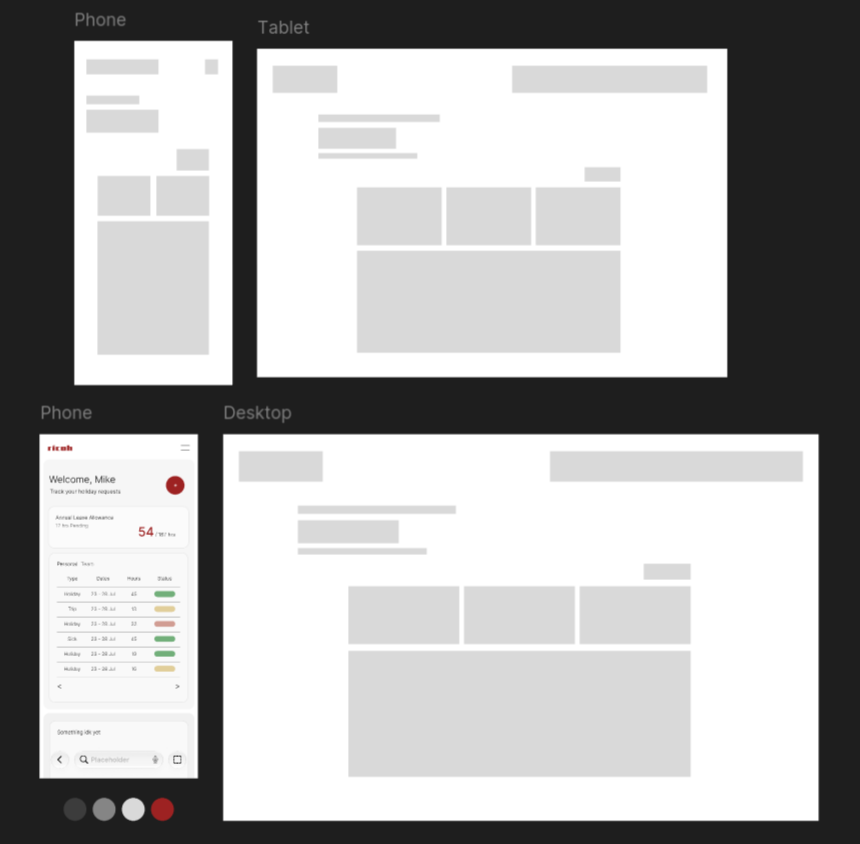
\includegraphics[width=12cm]{media/designs.png}
  \caption{Application Wireframes \& High Fidelity}
  \label{fig:designs}
\end{figure}

As displayed in Figure~\ref{fig:designs} the application's main content is located in the centre of the visible space, with the logo and navigation on the top.
Horizontal navigation on the top, provides an optimal and familiar location for users, as well as enables more space for components.
High Fidelity diagram created to showcase potential final website interface, with colour, shadows, borders and placeholder text.

\subsubsection{Agile}
Designs were shared with group, displaying wireframes for different device formats as well as a high fidelity design.
Feedback was limited due to the early stage of the overall development cycle.
This sprint's duration exceeded initial time expectations, due to \nameref{appendices:subsub:analysis-paralysis} (Appendices), concluding with a simple design to improve after the application meets original requirements.

\pagebreak{}

\subsection{Sprint 2: Backend Improvements}
Postgres Database and API required updating to enable token refreshing, a logout option and overall improvements.
New improvements improve user experience by storing refresh tokens, preventing the user from mandatory login after certain duration. 

\subsubsection{Database}
Created 'refresh\_token' and 'invalidated\_jti' tables to provide reference for the API to determine user authorisation.

\subsubsection{API}
Developed a token API service providing CRUD functions for user refresh and invalidated access tokens table records.
Enabled CORS to allow communication between the backend API and the React application.
Login endpoint was updated to return the refresh token alongside the JWT, and the JWT expiration time was reduced to 2 minutes to strengthen security.
This may be further improved by passing the refresh token directly into a http only cookie on login, instead of manually assigning a cookie in the React application.
Additionally, cookie-based handling was enabled, and implemented at a new logout endpoint to check the cookie stored refresh token and delete the relavent associated 'refresh\_token' record from the database.

\subsubsection{Agile}
\pagebreak{}

\subsection{Sprint X: Further}
Add a log component in the admin to see errors and so on, need to modify api.
test on other browsers
\pagebreak{}


\section{Notes}
- refresh token tbl could also contain a refreshed\_on column for more analytics \\
- refresh token rn is passed in jwt, this can be improved - send refresh token as cookie http only

Items to complete withiin this
code design, creaiton, developemnt plan, sprint conclusion, testing for each sprint

right now the access token will be manually set as a cookie in react, this can be improved in the api by also attatching the jwt to a cookie


\subsection{Application Designs}
- wireframes
- hi/lo \\
holiday page, requests page, admin page

\subsection{Testing}

\subsection{Security}

Access and refresh tokens used. Jwt
on log out, the refresh token needs to be invalidated - this can be by adding a revoked at column, or deleting the refresh token record entirely, forcing the user to log in and create one.
the expires at column could also be used to accomadte this, however this overloads the objective, and purpose as well as the identity of that column.
For simplicity, user records are deleted on log out. 

\pagebreak
\section{Appendices}

\subsection{User Exerience/Interface}

\subsection{Analysis Paralysis}
\label{appendices:subsub:analysis-paralysis}

\subsection{Git}
\subsection{Agile}
\subsection{Testing}
\subsection{Rendering Models}
\subsection{React}
\subsection{Tokens}
\subsection{Web Storage}

cookies and jwt, vs local storage, data being in jwt, manipulation, 


\end{document}
